\documentclass[]{article}
%\usepackage{lmodern}
\usepackage{amssymb,amsmath}
\usepackage{ifxetex,ifluatex}
\usepackage{fixltx2e} % provides \textsubscript
\ifnum 0\ifxetex 1\fi\ifluatex 1\fi=0 % if pdftex
  \usepackage[T1]{fontenc}
  \usepackage[utf8]{inputenc}
\else % if luatex or xelatex
  \ifxetex
    \usepackage{mathspec}
    \usepackage{xltxtra,xunicode}
  \else
    \usepackage{fontspec}
  \fi
  \defaultfontfeatures{Mapping=tex-text,Scale=MatchLowercase}
  \newcommand{\euro}{€}
\fi
% use upquote if available, for straight quotes in verbatim environments
\IfFileExists{upquote.sty}{\usepackage{upquote}}{}
% use microtype if available
\IfFileExists{microtype.sty}{%
\usepackage{microtype}
\UseMicrotypeSet[protrusion]{basicmath} % disable protrusion for tt fonts
}{}
\usepackage{graphicx}
\makeatletter
\def\maxwidth{\ifdim\Gin@nat@width>\linewidth\linewidth\else\Gin@nat@width\fi}
\def\maxheight{\ifdim\Gin@nat@height>\textheight\textheight\else\Gin@nat@height\fi}
\makeatother
% Scale images if necessary, so that they will not overflow the page
% margins by default, and it is still possible to overwrite the defaults
% using explicit options in \includegraphics[width, height, ...]{}
\setkeys{Gin}{width=\maxwidth,height=\maxheight,keepaspectratio}
\ifxetex
  \usepackage[setpagesize=false, % page size defined by xetex
              unicode=false, % unicode breaks when used with xetex
              xetex]{hyperref}
\else
  \usepackage[unicode=true]{hyperref}
\fi
\hypersetup{breaklinks=true,
            bookmarks=true,
            pdfauthor={},
            pdftitle={Consequentialism},
            colorlinks=true,
            citecolor=blue,
            urlcolor=blue,
            linkcolor=magenta,
            pdfborder={0 0 0}}
\urlstyle{same}  % don't use monospace font for urls
\setlength{\parindent}{0pt}
\setlength{\parskip}{6pt plus 2pt minus 1pt}
\setlength{\emergencystretch}{3em}  % prevent overfull lines
\setcounter{secnumdepth}{0}

\title{Consequentialism}
\date{}

\begin{document}
\maketitle

\subsection{Consequentialism}\label{consequentialism}

\begin{figure}[htbp]
\centering
%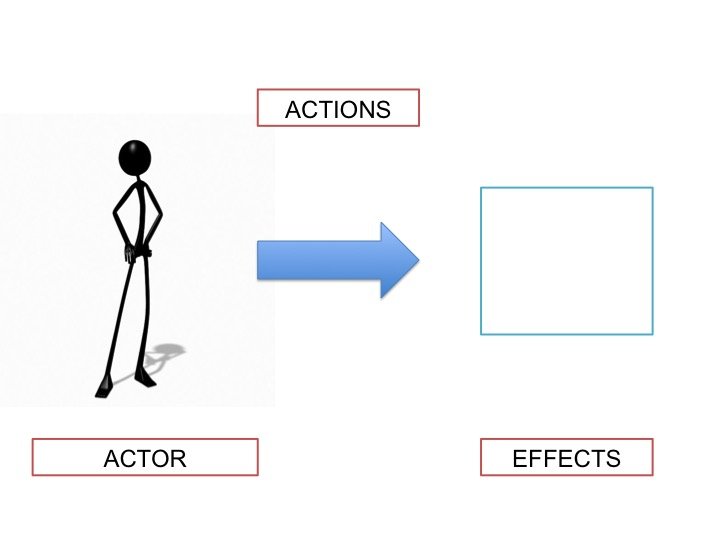
\includegraphics{/Teaching/Examined/Ethics/Slide1.jpg}
\caption{alt text}
\end{figure}

Consequentialists claim that morality depends completely on the effects
of our actions. They say that the actor side of the diagram is
irrelevant as is the intrinsic nature of their acts.

There are different versions of Consequentialism. They differ,
primarily, in what effects they construe as relevant for morality.
\textbf{Egoism} says that right actions are those that further one's own
best interests. Egoists say that the effects your actions have on others
is irrelevant to the morality of your actions. All that is relevant is
the effects your actions have on you. For further discussion of egoism,
see the textbook.

\subsection{Utilitarianism}\label{utilitarianism}

In this handout, I will discuss a second version of Consequentialism.
\textbf{Utilitarianism} agrees that the effects of an action determines
its morality. Unlike the egoist, the utilitarian claims that the effects
actions have on everyone (including yourself) is what determines their
morality. On this view, your action may harm your self interest, but
will still be right if the positive effects of the action on others
outweighs the harms to yourself. Utilitarians accept the following
principle:

\begin{description}
\itemsep1pt\parskip0pt\parsep0pt
\item[The Principle of Utility]
Rights actions are those that result in greater overall well-being (or
utility) for the people involved than any other possible action.
\end{description}

Consider torture. The police learn that a person S has planted a bomb
somewhere in the city. They arrest S who remains silent after intense
questioning. A police officer asks herself, `would it be morally
permissible for me to force an answer using violence, using torture?'
The utilitarian denies that there are is an absolute moral prohibition
against torture. Whether it is moral depends entirely on the effects the
action will have on the people involved.

What effects should we attend to? Utilitarians disagree on this point.
For our purposes, we can focus on Jeremy Bentham's rather simple view
that the only effects that matter are the pleasures and pains caused by
the action on the people involved. On this view, one should maximize
pleasure and minimize pains regardless of the distribution of those
pleasures and pains. Here we have to consider two scenarios:

\begin{description}
\itemsep1pt\parskip0pt\parsep0pt
\item[Scenario 1]
The police officer tortures the prisoner. The prisoner experiences much
pain. The officer suffers mental torment. The bomb is found. The officer
feels relief at preventing a tragedy. Nobody suffers the pain of being
injured, maimed by an exposition. Nobody suffers the pain from dying in
an explosion. Nobody suffers the pain of losing a loved one in an
explosion.
\item[Scenario 2]
The police officer does not torture the prisoner. The prisoner suffers
no physical pain. The officer suffers no mental anguish from torturing
her prisoner. Several people suffer incredible pain from being injured
in the explosion. Many suffer great pain as they die from the explosion.
Many suffer great pain from losing a loved one.
\end{description}

The officer can torture or not. According to utilitarianism, she should
decide by comparing the prospective pleasures and pains involved in both
scenarios. As presented, scenario 2 involves a far greater ratio of pain
to pleasure than scenario 1. Suppose that we quantify pains and
pleasures. Scenario 1 might result in 20 units of pain and 20 units of
pleasure, which is a ratio of pain to pleasure of 1:1. Scenario 2 might
result in 2000 units of pain and 10 units of pleasure, which is a ratio
of pain to pleasure of 200:1. Clearly the first scenario has a better
ratio of pain to pleasure, so, according to the utilitarian, torture is
the morally required thing to do in this circumstance.

\subsection{Rule vs.~Act
Utilitarianism}\label{rule-vs.act-utilitarianism}

Utilitarianism may seem to legitimize such terrible evils that it is
unworthy of our attention. If the choice is between a huge amount of
pleasure for a small group of people or a very small amount of pleasure
for a huge number of people, we should advance the interest of the
minority. Among other things, this legitimizes slavery if the benefits
to the slave owners far outweigh the pain suffered by the slaves. A
terrible result! Utilitarianism, though, is a much more sophisticated
theory than it first appears. There are two very distinct versions of
it:

Act-utilitarianism: : The rightness of actions depends solely on the
overall well-being produced by individual actions.

Rule-utilitarianism: : A right action is one that conforms to a rule
that, if followed consistently, would create for everyone involved the
most beneficial balance of well-being over suffering.

Act Utilitarianism has the unpleasant results I just mentioned. It says
that the rightness and wrongness of an \emph{individual action} depends
solely on the overall well-being produced by that \emph{individual act}.
Torture in a particular situation is moral because that individual act
of torture produces a greater balance of well-being over suffering than
any alternative action. In a different circumstance, an individual act
of torture is immoral because that individual act produces a worse
balance of well-being over suffering that some alternative. Act
utilitarianism, then, says that an individual act should be isolated
from similar acts and evaluated merely on the basis of that individual
act's effects.

Rule Utilitarianism, on the other hand, says that an individual act
cannot be isolated from similar acts. It claims that the rightness and
wrongness of an act depends on the effects that would be produced by
everyone doing similar acts, i.e., by following a rule that sanctioned
or prohibited that act.

Note that adhering to certain rules to maximize well-being for everyone
involved may require us to perform particular acts that have bad effects
in a particular situation. Consider our torture case once again.

\begin{description}
\itemsep1pt\parskip0pt\parsep0pt
\item[Scenario 1]
The police officer tortures the prisoner. Here the officer is acting as
if it is generally permissible for the police to torture prisoners. What
would the effects of this permission being granted to the police force?
On the one hand, they may stop some crimes using that torture. Perhaps
they will catch a guilty party or two. But this will be far out shadowed
by the turmoil that would ensue. Riots would follow. Few, if any, would
report a crime or cooperate with the police.
\item[Scenario 2]
The police officer does not torture the prisoner. Here the officer is
acting on the assumption that it is never permissible for the police to
torture a prisoner. Here the prisoner suffers no physical pain. The
officer suffers no mental anguish from torturing her prisoner. There is
no civil strife from a corrupt police force which has not lost the trust
of the public. Nevertheless, several people suffer incredible pain from
being injured in the explosion. Many suffer great pain as they die from
the explosion. Many suffer great pain from losing a loved one.
\end{description}

Here we must assess the effects of both rules being implemented and
followed. In Scenario 1, the negative effects may involve a breakdown in
civil society. In Scenario 2, civil society is preserved but several
acts of terrorism may not be prevented. Nevertheless, the negative
effects in Scenario 1 likely outweigh those in Scenario 2. Thus the Rule
Utilitarian will judge it immoral to torture even though, on occasion,
it might help us avoid some specific negative result.

For more on utilitarianism, watch the following series of
\href{https://www.youtube.com/watch?v=uvmz5E75ZIA\&list=PLtKNX4SfKpzWiiUdXS9MKf8bgUfQSOlas}{clips.}

\end{document}
